\documentclass[tikz,margin=.1in]{standalone}
\usepackage{pgfplots,lmodern}
\pgfplotsset{compat=newest}

\begin{document}
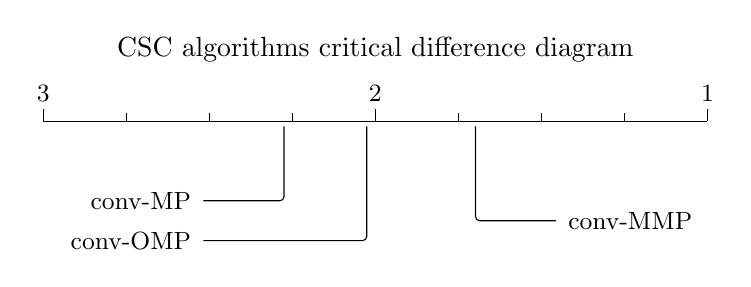
\begin{tikzpicture}[
  treatment line/.style={rounded corners=1.5pt, line cap=round, shorten >=1pt},
  treatment label/.style={font=\small},
  group line/.style={ultra thick},
]

\begin{axis}[
  clip={false},
  axis x line={center},
  axis y line={none},
  axis line style={-},
  xmin={1},
  ymax={0},
  scale only axis={true},
  width={\axisdefaultwidth},
  ticklabel style={anchor=south, yshift=1.3*\pgfkeysvalueof{/pgfplots/major tick length}, font=\small},
  every tick/.style={draw=black},
  major tick style={yshift=.5*\pgfkeysvalueof{/pgfplots/major tick length}},
  minor tick style={yshift=.5*\pgfkeysvalueof{/pgfplots/minor tick length}},
  title style={yshift=\baselineskip},
  xmax={3},
  ymin={-2.5},
  height={3\baselineskip},
  xtick={1,2,3},
  minor x tick num={3},
  x dir={reverse},
  title={CSC algorithms critical difference diagram},
]

\draw[treatment line] ([yshift=-2pt] axis cs:1.69859375, 0) |- (axis cs:1.44859375, -2.5)
  node[treatment label, anchor=west] {conv-MMP};
\draw[treatment line] ([yshift=-2pt] axis cs:2.02609375, 0) |- (axis cs:2.5253125, -3.0)
  node[treatment label, anchor=east] {conv-OMP};
\draw[treatment line] ([yshift=-2pt] axis cs:2.2753125, 0) |- (axis cs:2.5253125, -2.0)
  node[treatment label, anchor=east] {conv-MP};

\end{axis}
\end{tikzpicture}
\end{document}
